\section{Literature Review}

Fabric classification has gained interest within computer vision and material science, with applications across many industries, including fashion, healthcare, manufacturing, and forensics. The advancements in deep learning have enabled researchers to develop automated approaches that accurately recognize and classify textile materials using image data. 

The traditional process of fabric classification has relied on manual methods and physical methods. Processes which are time-consuming, subjective to human error, and require equipment that could be specialized. The image-based classification of textiles and fabrics using deep learning models offers a more scalable and efficient approach and would allow for real-time implementations. 

In this section, we present key research contributions that have applied deep learning approaches to fabric classification because the datasets highlighted here (as used in these studies), are carefully considered when describing the research, as data quality and diversity are important when developing models that will be having a good performance. We also provide a detailed description of the three papers selected and implemented as part of this research work. Each paper takes a different modelling approach to highlight the merits and limitations of the current methodologies.

Through the exploration of all these work, we look to illuminate shared practices, inventive ideas, and existing issues in the domain, which have helped inform our proposed methodology.

\subsection{Dataset Overview}

The implementation and level of understanding of a strong, efficacious and generalized deep learning model that classifies fabrics is tied to the availability of high-quality, heterogeneous, and well-structured datasets. Each of the datasets provided in this domain provides textile properties from a fixed standpoint - with some focusing on fine surface-level textures, others providing microscopic or structural imaging, and others providing extensive predominately labeling through expert-based functional taxonomies.

Here, we provide our overview and review of three datasets which we utilized in the development and audit of our deep learning models for this research. These datasets were selected based upon relevance, heterogeneity, and the diversity of challenges that they represent in the fabric classification domain. Each dataset has helped inform our understanding of how fabrics presented visually, micro-structure, and material properties can be categorized in these helpful analyses. The datasets reviewed are described below:

\subsubsection{A. Fine-Grained Material Classification Using Micro-geometry and Reflectance~\cite{kampouris2016fine}}

One of the important base datasets for fine-grained material classification is based on detailed geometry and reflectance properties, introduced by Kampouris et al., which highlights slightly different materials through high-resolution images of shape, surface details, and reflections captured under different lighting conditions.

The dataset was captured using a custom-built photometric stereo sensor designed to acquire fine surface details of fabric materials. Each sample in the dataset corresponds to a small patch of fabric, captured under four different illumination conditions to facilitate the extraction of both micro-geometry (surface normals) and reflectance (albedo).

The dataset consists of several classes of fabrics that are listed in Table~\ref{tab:fabric_distribution}. Each class contains multiple samples, with each sample having four images corresponding to different light sources.

\begin{table}[H]
\centering
\caption{Fabric-wise Distribution of Samples and Images}
\label{tab:fabric_distribution}
\begin{tabular}{|l|c|c|}
\hline
\textbf{Fabric Class} & \textbf{Number of Samples} & \textbf{Total Images} \\
\hline
Acrylic & 12 & 48 \\
Artificial Fur & 1 & 4 \\
Artificial Leather & 3 & 12 \\
Blended & 411 & 1,644 \\
Chenille & 13 & 52 \\
Corduroy & 24 & 96 \\
Cotton & 588 & 2,352 \\
Crepe & 26 & 104 \\
Denim & 162 & 648 \\
Felt & 4 & 16 \\
Fleece & 33 & 132 \\
Leather & 16 & 64 \\
Linen & 19 & 76 \\
Lut & 4 & 16 \\
Nylon & 57 & 228 \\
Polyester & 226 & 904 \\
Satin & 24 & 96 \\
Silk & 50 & 200 \\
Suede & 5 & 20 \\
Terrycloth & 30 & 120 \\
Unclassified & 123 & 492 \\
Velvet & 11 & 44 \\
Viscose & 37 & 148 \\
Wool & 90 & 360 \\
\hline
\textbf{Total} & \textbf{2,048} & \textbf{8,192} \\
\hline
\end{tabular}
\end{table}


\begin{itemize}[noitemsep, topsep=0pt]
    \item \textbf{Images per sample:} 4 RGB images (one per light source)
    \item \textbf{Original resolution:} 640$\times$640 pixels
    \item \textbf{Cropped resolution:} 400$\times$400 pixels (to avoid out-of-focus regions)
    \item \textbf{Field of View:} Approximately 10 mm $\times$ 10 mm
    \item \textbf{Working Distance:} 3 cm - Distance from the camera to the fabric sample
\end{itemize}

\begin{figure}[H]
    \centering
    \begin{minipage}{0.8\linewidth}
        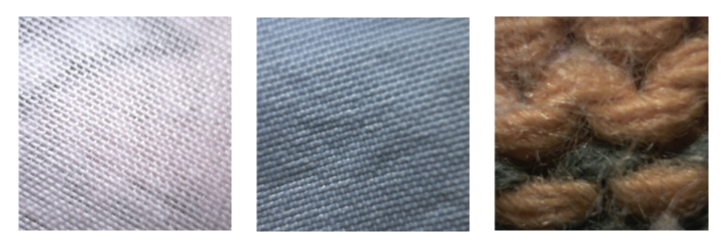
\includegraphics[width=\linewidth]{images/iBugDataset}
    \end{minipage}
    \caption[Sample images from the iBug Fabric Dataset]{Sample images from the iBug Fabric Dataset: (Left) Cotton, (Middle) Polyester, (Right) Wool.}
\end{figure}

\subsubsection{B. Optical Coherence Tomography Image Dataset of Textile Fabrics~\cite{sabuncu2022optical}}

The Optical Coherence Tomography (OCT) image dataset of textile fabrics is a distinct and specialized dataset comprised of high-resolution cross-sectional images of fabric structures. The dataset was produced by Sabuncu and Ozdemir, and thus far, has been used to support material classification tasks through depth imaging. Specifically, it has been helpful in textile engineering, recycling, and forensic investigations. 

The dataset includes OCT scans of fabrics made of only cotton, wool, and polyester. To accomplish this, three samples were taken from each of the three material types (cotton, wool, polyester) resulting in nine fabric types total. Each sample was scanned using the Thorlabs CAL110C1 OCT system over 100 random places on the surface of the sample with the objective of generating high-quality cross-sectional images or B-scans. The scans are all 2mm long and were excluded from other filtering options or pre-processing protocols, and were saved in raw \texttt{.png} images.

\begin{table}[H]
\centering
\caption{Class-wise image distribution of the Fabric OCT Dataset}
\begin{tabular}{ll}
\toprule
\textbf{Fabric Type} & \textbf{Number of images} \\
\midrule
Cotton & 495 \\
Polyester & 448 \\
Wool & 533 \\
\bottomrule
\end{tabular}
\end{table}

One of the main benefits of OCT imaging is that it shows aspects of a fabric’s internal microstructure that would be impossible to see from a standard RGB image: weave pattern, layer thickness, and material density internal to the fabric can provide great utility for classifying fabrics that may look the same on the surface. 

\begin{figure}[H]
    \centering
    \begin{minipage}{0.8\linewidth}
        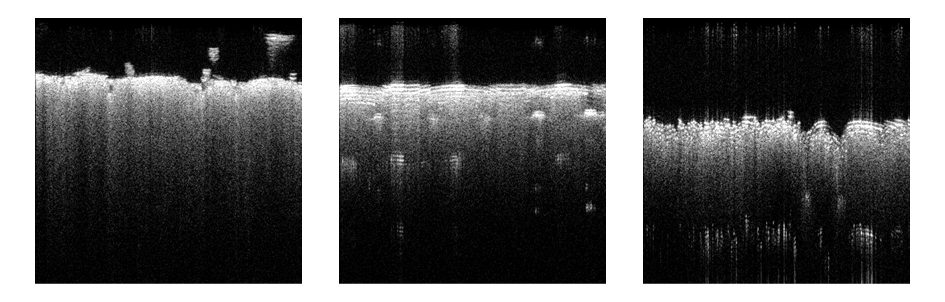
\includegraphics[width=\linewidth]{images/FabricOCTDataset.png}
    \end{minipage}
    \caption[Sample images from the Fabric OCT Dataset]{Sample images from the Fabric OCT Dataset: (Left) Cotton, (Middle) Polyester, (Right) Wool.}
\end{figure}

The dataset used in this project was organized into three folders, cotton, wool, and polyester, with multiple scans of different fabric pieces made from the same material per folder. A dataset organized this way is well-labeled and clean, supporting the training and testing of deep learning models, model architectures that will most likely learn from structural features rather than appearance. 

In summary, the OCT image dataset has a high degree of uniformity and detail, making it highly suitable for fine-grained classification of fabrics according to their internal structure. Additionally, its potential goes beyond classification, applications include recycling, identifying defects in textiles, and suitable for automated textile quality control assessments.

\subsubsection{C. TextileNet: A Material Taxonomy-Based Fashion Textile Dataset~\cite{zhong2023textilenet}}

TextileNet is a large-scale taxonomy-based dataset with the aim of facilitating textile material identification through deep learning methods. Originally proposed by Shu Zhong et al., TextileNet fills a significant gap that currently exists in datasets by providing a taxonomy of textile materials in a logical form covering two main branch of fibres and fabrics. In contrast to most datasets in the area of fashion that are poorly annotated and only provide mixed labels for fabric and fibre, or offer loose, ambiguous labels, TextileNet's labels are clearly defined with a scientific basis provided by material science researchers.

TextileNet consists of two datasets: \textit{TextileNet-fibre} and \textit{TextileNet-fabric}, with 33 fibre labels and 27 fabric labels included in the datasets. The combined dataset has approximately 760,949 images collected from Google Images and reconstituted fashion datasets such as iMaterialist. The images were collected based on keywords from subsequent queries which were derived from the defined textile taxonomy ensuring that the data collected conveys the type of real-world clothing items, but consistently added images in the same area across the project archive.

\begin{figure}[H]
    \centering
    \begin{minipage}{0.8\linewidth}
        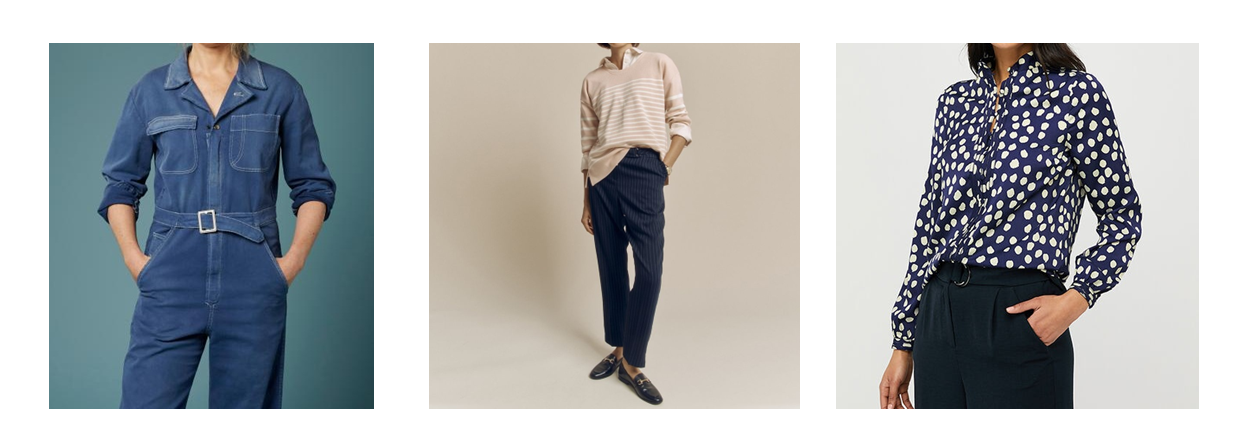
\includegraphics[width=\linewidth]{images/TextileNetDataset.png}
    \end{minipage}
    \caption[Sample images from the TextileNet Dataset]{Sample images from the TextileNet Dataset: (Left) Denim, (Middle) Crepe, (Right) Satin.}
\end{figure}

The value of TextileNet lies in its taxonomy-based structure. The fibre taxonomy range from natural, synthetic, and regenerated fibres (eg cotton, wool, polyester, bamboo viscose and milk casein). While the fabric taxonomy provides categories based on the methods of production (woven, knitted, non-woven), each with its examples (denim, tweed, velvet, jersey).

Overall, TextileNet is suitable for training efficient models for complex fabric composition recognition for both retail, recycling, supply chain application and as support to sustainable fashion design.

\subsection{Existing Work}

In recent years, deep learning has shown remarkable progress in image-based classification tasks across various domains, including textiles. Numerous research efforts have applied Convolutional Neural Networks (CNNs) and Transformer-based architectures to classify fabrics and textile compositions with increasing accuracy and robustness. The integration of transfer learning and custom dataset preparation has further improved the performance of these models, even when working with limited or domain-specific data.

This section focuses on the review of selected research papers that have been implemented as part of this thesis. These papers represent different approaches to fabric classification—ranging from traditional CNN models to more advanced hybrid pipelines involving Vision Transformers and statistical techniques like Principal Component Analysis (PCA) and Linear Discriminant Analysis (LDA).

Each study has contributed significantly to the understanding of fabric classification challenges and techniques. By implementing and analyzing these works, we gain insights into the strengths and limitations of various deep learning models when applied to textile data. The outcomes from these implementations also provide the foundation for designing a more effective and efficient hybrid model tailored to the requirements of fine-grained fabric recognition.

\subsubsection[A. Research on Classification of Clothing Fabrics Images Based on Convolutional Neural Network]{A. Research on Classification of Clothing Fabrics Images Based on Convolutional Neural Network~\cite{hong2024research}}

In the paper \textit{“Research on Classification of Clothing Fabrics Images Based on Convolutional Neural Network”} by Ying Hong et al., the authors propose a deep learning-based approach to automatically classify clothing fabric types using image data. The main motivation behind the study is the growing need for intelligent fabric identification systems in clothing design and textile production, where manual classification can be time-consuming and inconsistent.

The authors utilize a transfer learning strategy by fine-tuning the VGG-16 model, a well-established convolutional neural network architecture, pre-trained on the ImageNet dataset. The study focuses on a custom dataset composed of 15,000 high-resolution images representing 10 different types of clothing fabrics, including cotton, wool, silk, denim, and others. The images are captured under controlled lighting conditions to ensure consistency and minimize background noise.

\begin{figure}[H]
    \centering
    \begin{minipage}{1\linewidth}
        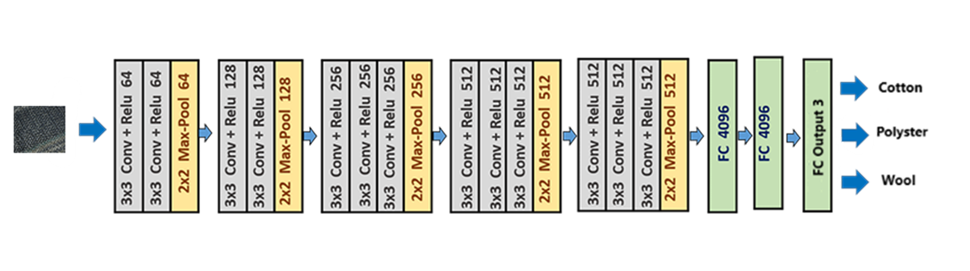
\includegraphics[width=\linewidth]{images/Paper1Model.png}
    \end{minipage}
    \caption[Model architecture - Hong et al.~\cite{hong2024research}]{Model architecture used for classification in Hong et al.~\cite{hong2024research}.}
\end{figure}

To enhance model generalization, the dataset undergoes data augmentation using techniques such as rotation, flipping, brightness adjustment, and the addition of Gaussian noise. These transformations help the network learn invariant features and reduce the risk of overfitting.

The proposed model achieves a test accuracy of 99.73\%, demonstrating high performance in distinguishing between visually similar fabric types. The authors also emphasize the model’s fast convergence rate and robust classification capabilities, suggesting that convolutional networks, even with moderate architectural depth like VGG-16, can be effectively employed for practical fabric recognition tasks.

This work highlights the advantages of combining transfer learning with carefully curated datasets and simple preprocessing steps. It confirms that CNN-based methods are well-suited for fabric classification, especially when high-quality image data is available. Additionally, the study provides a foundation for future research to explore more advanced architectures or multi-modal data sources, such as combining texture with reflectance or depth information.

\subsubsection[B. TextileNet: A Deep Learning Approach for Textile Fabric Material Identification from OCT and Macro Images]{B. TextileNet: A Deep Learning Approach for Textile Fabric Material Identification from OCT and Macro Images~\cite{siam2023textilenet}}

In the paper \textit{“TextileNet: A Deep Learning Approach for Textile Fabric Material Identification from OCT and Macro Images”} by Siam et al., the authors explore the use of deep learning models for automatic fabric material identification using two distinct types of images: macro images and Optical Coherence Tomography (OCT) scans. This work addresses the challenge of accurately classifying fabrics such as cotton, wool, and polyester, which often appear visually similar to the human eye but have distinct structural properties.

\begin{figure}[H]
    \centering
    \begin{minipage}{1\linewidth}
        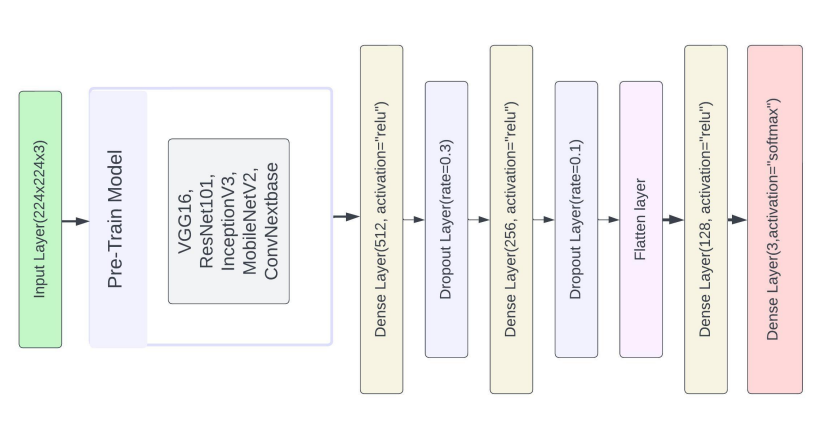
\includegraphics[width=\linewidth]{images/Paper2Model.png}
    \end{minipage}
    \caption[Model architecture - Siam et al.~\cite{siam2023textilenet}]{Model architecture used for fabric classification in Siam et al.~\cite{siam2023textilenet}}
\end{figure}

The study introduces a classification pipeline based on transfer learning, utilizing five pre-trained convolutional neural networks: MobileNetV2, VGG16, ResNet101, InceptionV3, and ConvNextBase. These models were adapted and fine-tuned to classify textile samples based on their visual and structural features.

To improve image quality and enhance model performance, preprocessing techniques such as grayscale conversion, contrast enhancement (CLAHE), and sharpening were applied. All images were resized to a standard input size of 224×224 pixels before being fed into the models.

The results demonstrate that MobileNetV2 outperformed the other models, achieving 99.87\% accuracy on OCT images and 95.17\% accuracy on macro images. The significant difference in performance between the two image types highlights the added value of using OCT imaging for fabric classification, as it reveals deeper structural features not visible in surface-level macro images.

This work shows that combining deep learning with high-resolution image modalities like OCT can lead to highly accurate and reliable fabric classification. The proposed pipeline is lightweight and efficient, making it suitable for real-world applications in the textile industry, such as automated material sorting, quality control, and textile recycling.

\subsubsection[C. Fabric Composition Identification using Fine-Tuned Vision Transformers]{C. Fabric Composition Identification using Fine-Tuned Vision Transformers~\cite{chitra2023fabric}}

The study \textit{“Fabric Composition Identification using Fine-Tuned Vision Transformers”} by Chitra G M et al. presents a modern approach to fabric classification by leveraging the capabilities of Vision Transformers (ViTs). Unlike traditional methods that rely solely on convolutional features, this work incorporates transformer-based architectures to extract and understand both local and global features in fabric images. The main goal of the study is to identify fabric compositions, especially in scenarios where fabrics may contain blends of multiple fibres.

The dataset used in the study consists of 937 images, each labeled with fabric compositions such as cotton, polyester, nylon, and silk. The images were captured using smartphone cameras, simulating a real-world setting where users or retailers may need to classify fabric types using accessible devices. This practical setup makes the proposed method more adaptable for mobile or on-site fabric recognition applications.

The proposed pipeline combines several stages. Initially, features are extracted from images using a fine-tuned ViT model. These features are then reduced using Principal Component Analysis (PCA) and further refined using Linear Discriminant Analysis (LDA) to enhance class separation. Finally, a Support Vector Machine (SVM) classifier is used for the final prediction. The authors also apply Platt scaling to calibrate the probability outputs of the SVM for better confidence estimation.

\begin{figure}[H]
    \centering
    \begin{minipage}{1\linewidth}
        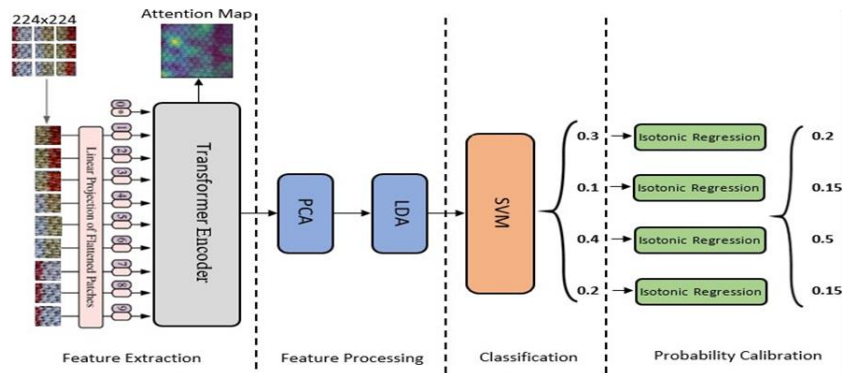
\includegraphics[width=\linewidth]{images/Paper3Model.png}
    \end{minipage}
    \caption[Model architecture - Chitra G M et al.~\cite{chitra2023fabric}]{Model architecture used for fabric composition identification in Chitra G M et al.~\cite{chitra2023fabric}}
\end{figure}

The model achieves an average F1-score of 0.87, along with a mean squared error (MSE) of 0.20 and a log-loss of 0.44. These results show that the pipeline is capable of reliably identifying both pure and mixed fabric types. Additionally, the use of SHAP (SHapley Additive exPlanations) values provides interpretability to the model by highlighting which parts of the image influenced the classification decision. This is especially useful in understanding how the model distinguishes between blended materials.

Overall, this work demonstrates the potential of Vision Transformers in fabric composition analysis. Its hybrid approach—combining ViTs with traditional dimensionality reduction and machine learning classifiers—offers a practical solution for real-world applications, including quality assurance, textile recycling, and online garment classification.
